\documentclass[10pt,a4paper]{article}
\usepackage[margin=22mm]{geometry}
\usepackage{amsmath,amssymb,amsthm,booktabs,longtable,array,graphicx,xcolor,enumitem,microtype}
\usepackage[colorlinks=true,linkcolor=blue!45!black,urlcolor=blue!55!black,citecolor=blue!45!black]{hyperref}
\hypersetup{pdftitle={Acquiring an Optimal Productive Controller Without Acquiring Its Rare-Failure Value},pdfauthor={Astra research continuation},pdfsubject={Conditional control theorems, finite certificates and physical resource boundaries}}
\usepackage{fancyhdr}
\pagestyle{fancy}\fancyhf{}\fancyhead[L]{Acquired productive control}\fancyhead[R]{5 November 2026}\fancyfoot[C]{\thepage}
\setlength{\headheight}{13pt}\setlength{\parskip}{4pt}\setlength{\parindent}{0pt}
\setlist{nosep,leftmargin=*}
\newtheorem{theorem}{Theorem}\newtheorem{proposition}{Proposition}
\newcommand{\E}{\mathbb E}\newcommand{\Pp}{\mathbb P}
\newcommand{\kl}{\operatorname{kl}}\newcommand{\KL}{\operatorname{KL}}
\title{Acquiring an Optimal Productive Controller\\Without Acquiring Its Rare-Failure Value}
\author{Astra research continuation\\Conditional theorems, finite certificates and physical limits}
\date{5 November 2026}
\begin{document}
\maketitle
\begin{abstract}
We construct a finite experimental certificate for an entire feedback policy when interventions change the failure and recovery law. The objective is completed useful output before service failure. For a declared class of controlled nearest-neighbor damage processes, local uncertainty inequalities certify a policy optimal among every allowed randomized and history-dependent controller, from every safe state and for every failure threshold. In a stable parameter region, the evidence and policy description are independent of the damage-buffer depth, although expected useful output grows exponentially with depth and an absolute relative-value forecast requires quadratically growing evidence. The certificate also covers arbitrary fixed state-dependent transition rows inside uniform action envelopes; constant-cost acquisition of those envelopes requires a separate homogeneity or physical-transfer premise.

A distinct finite-mission certificate tolerates history-dependent drift inside conditional bounds. A matching information obstruction shows why an unassayed intervention-specific catastrophic channel can restore rare-event acquisition costs. An independently developed productive repair model supplies an attained capacity boundary and exact energy, repair-stock and shared-support limitations. The mechanism uses established skip-free dynamic programming, stochastic comparison and statistical change of measure. Historical novelty and a civilisation-changing capability are not established. The execution uses simulated finite records and exact rational checks; no hardware experiment is claimed.
\end{abstract}
\setcounter{tocdepth}{1}
{\small\tableofcontents}
\newpage

\section{Selected question and completed endpoint}

The selected question is: \emph{Can finite local evidence certify the complete optimal productive feedback rule, even when the rule changes the failure law and the value of operating it remains difficult to predict?} The indispensable operation is an action-optimality certificate that does not first require an accurate rare-event value function.

The completed endpoint is a mathematical acquisition-and-control theorem at a finite-cycle interface, with an executable compiler and an independent verifier. It moves beyond selecting a kinetic menu under one invariant law: it optimizes positive useful output over every admissible feedback policy, permits changed invariant laws, and obtains one policy valid across an unbounded family of failure thresholds. It does not provide a general physical prevention device or establish the device contract from arbitrary short traces.

Three routes were constructed independently. One developed productive birth--death control; one constructed an information obstruction with an attaining experiment; one derived the resource boundary of continuously productive repair. Their working proofs and checks are retained. Literature then exposed the core forward recursion as established machinery, especially Wijngaard and Stidham~\cite{wijngaard}. Structure-dependent policy identification is also established~\cite{zanette}. The claims here concern the specific finite uncertainty certificate, its acquisition and forecast comparison, its mission guarantee and its support boundary. No first-in-history claim follows from this search.

\subsection{Preserved context}

The preceding direct acquired-prevention package remains unchanged, including its common-invariant Gibbs construction, prediction lower bound, all-safe-start mean theorem, operating warm-up, grouped-wait assay, independent constructions and nested first-event machinery. The complete ZIP has 305 members, 7,338,297 bytes and SHA-256
\begin{quote}\small\ttfamily
5371d25f2caa2fd44ceb8d8cbef9c879589fdd03f12b649c68ba1e4507f1ae57.
\end{quote}
It contains the earlier receipt preserving all 229 files of the preceding first-event package. This return embeds that ZIP byte for byte and separately hashes all current deliverables.

P2's predictive-preparation source was read at the exact supplied revision~\cite{p2}:
\begin{center}\small\texttt{c11d35bd2e07116e214b4388302595cfedbd770e}\end{center}
It uses finite total energy, local dissipation, an LTI loaded plant and private random start times to obtain future-input prediction without hidden equilibration. None of those physical hypotheses implies the damage-process contract below. No unproved bridge between these classes is used. The shared methodological lesson is only that the necessary operation depends on the requested task.

\section{Finite physical interface and useful objective}

Let damage or outstanding-recovery count be $i\in\{0,\ldots,N\}$, with service failure at $N$. Each safe operating cycle has a finite fixed duration $\Delta$ and chooses one action from a finite menu $\mathcal A$. Sensing, action selection and waveform loading must fit inside the cycle. Action $a$ at safe state $i$ delivers verified useful output $r_i(a)>0$, then makes a transition
\begin{equation}
i\longrightarrow\begin{cases}i+1,&p_i(a),\\i-1,&q_i(a),\\i,&1-p_i(a)-q_i(a),\end{cases}
\qquad p_i(a)\ge p_{\min}>0,\quad q_i(a)\ge0,\quad p_i(a)+q_i(a)\le1 .
\label{eq:kernel}
\end{equation}
At zero, an attempted downward move reflects. The reward-before-transition convention ensures the reward in the terminal cycle is actually delivered. Other delivery conventions require the corresponding reward equation.

Every admitted action must meet a useful-throughput floor and finite power, waveform and resource bounds. This is the actual finite-cycle kernel, not a small-time approximation that silently omits multiple physical transitions. The structure could describe a suitably engineered repair backlog or cyclic degradation process; no particular apparatus has been shown to satisfy it.

Let $T_N$ count safe-start cycles through absorption and define
\begin{equation}
W_N=\sum_{t=0}^{T_N-1}r_{X_t}(A_t),\qquad
V_i^{(N)}=\sup_\pi\E_i^\pi W_N .
\label{eq:objective}
\end{equation}
Policies may use the complete observed past, private randomness and outputs, while choosing only allowed actions at cycle boundaries. This is a mean useful-work objective. Its optimizer need not maximize every deadline-survival probability or risk-sensitive utility. Hard total fuel, deadlines, state-dependent cycle lengths and switching costs change the problem.

The numerical probabilities describe actual operating conditions. Fixed Markov behavior, one-step transition support, adequate state observation, useful output and exclusion of separate catastrophic modes are premises. Ordinary finite transition records cannot certify those premises against unrestricted alternatives. Later sections give a precise obstruction, not just a qualitative warning.

\section{Exact operation: action choices from forward differences}

Define
\[
c_i(a)=\frac{r_i(a)}{p_i(a)},\qquad \rho_i(a)=\frac{q_i(a)}{p_i(a)}.
\]
Here $\rho$ compares repair with worsening; $c$ includes useful output and the pace of worsening.

\begin{theorem}[Forward useful-work verification]
Set
\begin{equation}
d_0=\max_a c_0(a),\qquad
d_i=\max_a\{c_i(a)+\rho_i(a)d_{i-1}\}\quad(i\ge1).
\label{eq:recursion}
\end{equation}
For every finite $N$ and safe initial state,
\begin{equation}
\boxed{V_i^{(N)}=\sum_{j=i}^{N-1}d_j.}
\label{eq:value}
\end{equation}
An action attaining the corresponding maximum is optimal at state $i$. One infinite state rule, restricted to states below $N$, is optimal for every $N$ and every safe initial distribution, among all admitted adaptive and randomized policies.
\end{theorem}

\begin{proof}
Conditional on any history, $N$ successive upward moves have probability at least $p_{\min}^N$. Thus every policy is absorbed with expected time at most $N/p_{\min}^N$. Bounded rewards on each finite state space give finite expectations.

Set $V_N=0$ and $V_i=\sum_{j=i}^{N-1}d_j$. At $i\ge1$ the inequality
$p_i(a)d_i\ge r_i(a)+q_i(a)d_{i-1}$ is exactly
\[
V_i\ge r_i(a)+p_i(a)V_{i+1}+q_i(a)V_{i-1}
+(1-p_i(a)-q_i(a))V_i.
\]
At zero use $p_0(a)d_0\ge r_0(a)$. Accumulated reward plus remaining $V$ is a supermartingale under any policy. Stop, then take the integrable absorption limit, to bound its expected reward by $V_i$. Maximizing actions attain equality at every step. The differences $d_i$ do not depend on terminal depth $N$.
\end{proof}

Forward recursion for skip-free controlled processes is established~\cite{wijngaard}; controlled birth--death and queueing problems have extensive precedent~\cite{serfozo}. The proof fixes the reward, initialization and policy quantifiers needed here.

\subsection{A finite controller across arbitrarily many thresholds}

For homogeneous action rows write $c_a,\rho_a$, with $f(d)=\max_a(c_a+\rho_a d)$. The map is increasing and convex; $d_i$ is nondecreasing. Along an increasing argument the active affine slopes can be chosen nondecreasing. Thus an optimal controller has at most $|\mathcal A|-1$ switches; each active action occupies one contiguous damage interval.

If $*$ has uniquely maximal $\rho_*>1$, put
\begin{equation}
D=\max_{a\ne *}\frac{(c_a-c_*)_+}{\rho_*-\rho_a}.
\label{eq:threshold}
\end{equation}
Above $D$, its line dominates every other line. Since
$d_i\ge c_*+\rho_*d_{i-1}$, some finite $m$ has $d_{m-1}>D$, and $*$ is optimal at all $i\ge m$. Neither $m$ nor this rule depends on $N$. A sufficient $m$ follows by comparing $D$ with $c_*(\rho_*^m-1)/(\rho_*-1)$.

The growth phases follow directly. If $\max_a\rho_a<1$, $f$ is a contraction with fixed point $d_\infty=\max_a c_a/(1-\rho_a)$, giving $V_0=Nd_\infty+O(1)$. If the maximum is one, the largest intercept among unit-slope actions eventually wins and $V_0$ is quadratic. If it exceeds one, the largest slope (largest intercept breaking ties) eventually wins and $V_0$ is exponential. These are consequences of the existing recurrence, not claimed as new drift theory.

\section{Finite uncertainty certificate for all depths}

Suppose evidence and physical transfer guarantees supply envelopes, at every state where used,
\begin{equation}
0<p_a^-\le p_i(a)\le p_a^+,\quad
0\le q_a^-\le q_i(a)\le q_a^+,\quad
0<r_a^-\le r_i(a)\le r_a^+ .
\label{eq:boxes}
\end{equation}
Let
\[
c_a^-=\frac{r_a^-}{p_a^+},\quad c_a^+=\frac{r_a^+}{p_a^-},
\qquad \rho_a^-=\frac{q_a^-}{p_a^+},\quad \rho_a^+=\frac{q_a^+}{p_a^-}.
\]
These may contain independently varying fixed rows at every damage level. No common invariant law or single homogeneous numerical generator is required for the certificate itself.

\begin{theorem}[A finite certificate for the entire optimal policy]
Certify a finite prefix $a_0,\ldots,a_{m-1}$ as follows. At zero require
$c_{a_0}^-\ge c_b^+$ for every competitor; set
$L_0=c_{a_0}^-$ and $U_0=c_{a_0}^+$. At each later prefix state require
\begin{equation}
\min_{d\in\{L_{i-1},U_{i-1}\}}
\big[(c_{a_i}^--c_b^+)+(\rho_{a_i}^--\rho_b^+)d\big]\ge0
\quad\text{for every }b\ne a_i,
\label{eq:prefix}
\end{equation}
then update $L_i=c_{a_i}^-+\rho_{a_i}^-L_{i-1}$ and
$U_i=c_{a_i}^++\rho_{a_i}^+U_{i-1}$.

Suppose a tail action $*$ has $\rho_*^->1$,
$\rho_*^->\max_{b\ne *}\rho_b^+$, and
\begin{equation}
L_{m-1}\ge D_{\rm box}:=
\max_{b\ne *}\frac{(c_b^+-c_*^-)_+}{\rho_*^--\rho_b^+}.
\label{eq:cone}
\end{equation}
Then the prefix followed by $*$ at every $i\ge m$ is exactly optimal for every fixed Markov model satisfying the envelopes, from every safe state and for every $N$.
\end{theorem}

\begin{proof}
Inductively the actual $d_i$ lies in $[L_i,U_i]$. The action comparison uses the \emph{same} preceding $d$, so its worst affine difference occurs at one interval endpoint. This proves the prefix test. Above $D_{\rm box}$ the lower tail line dominates all competitors' upper lines. Its update satisfies $c_*^-+\rho_*^-d\ge d$, so $[D_{\rm box},\infty)$ is invariant. Induction proves the infinite tail. Apply the forward verification theorem to each actual model and finite $N$.
\end{proof}

This certificate establishes choices without high-precision values of $d_i$ or $V_i$. It consists of a finite prefix and one invariant interval, with no catastrophic-trajectory probability estimation. Strict margins survive a nonzero neighborhood of local uncertainty. If comparisons remain unresolved, the procedure abstains; it does not certify arbitrary near-tie families.

\subsection{The acquisition premise is separate}

A homogeneous operating port can be tested at one safely prepared interior state. If probabilities can vary arbitrarily by state, untested tail rows cannot be bounded from that evidence. One must test all relevant rows, paying roughly linear row coverage and actual preparation, or earn a physical uniform envelope by another method. The robust theorem supplies neither transfer nor model completeness for free.

For a homogeneous port, reset the actual or justified matched specimen to state one, apply one complete operating cycle and classify up/down/hold. With $N\ge3$ this requires no catastrophe or near-failure preparation. Reset time, energy and fidelity remain charged. A reset does not itself reveal unknown parameters in the stated access model.

If each observed indicator has conditional bias at most $b$ relative to its target, $M$ trials per action give simultaneous intervals of half-width $h+b$ for all up/down probabilities, with total error at most
\begin{equation}
4|\mathcal A|e^{-2Mh^2}.
\label{eq:hoeffding}
\end{equation}
This follows from the bounded-increment Hoeffding argument and a union bound; up and down indicators within a trial need not be independent. Predictable bounded bias is required. Taking
$M\ge\log(4|\mathcal A|/\delta)/(2h^2)$ suffices. Positive certificate margins permit fixed $h$, independent of $N$.

With $K$ actions and prefix length $m$, the certificate procedure uses $O(Km)$ rational affine comparisons and updates. Finite encodings give finite integer payloads. The executed compiler implements the $m=1$ specialization, so it represents no large value function. One calibration event certifies every depth under the same envelope premise; reuse across depths does not incur a union bound over $N$. New equipment, age, operating conditions or expired calibration may demand new evidence. Systematic bias does not average away.

\section{A nontrivial family with changed failure laws}

The two nominal modes are
\begin{center}
\begin{tabular}{lrrrr}\toprule
Mode & Worsening $p$ & Repair $q$ & Hold & Useful output $r$\\\midrule
$A$ & $1/10$ & $1/5$ & $7/10$ & $3$\\
$B$ & $1/5$ & $7/10$ & $1/10$ & $2$\\\bottomrule
\end{tabular}
\end{center}
Both deliver at least two useful units per cycle. Mode $B$ has both greater worsening and much greater repair probability; it is not a rescaled clock. The reflected nonabsorbing chain has stationary adjacent-weight ratio $p/q=1/2$ under $A$ and $2/7$ under $B$. Their invariant laws differ.

The affine lines are $30+2d$ and $10+(7/2)d$. Mode $A$ wins at zero, and mode $B$ wins thereafter:
\begin{equation}
\pi^*(i)=\begin{cases}A,&i=0,\\B,&1\le i<N,\end{cases}
\qquad d_i=34(7/2)^i-4.
\end{equation}
Thus
\begin{equation}
\boxed{V_0^{(N)}=\frac{68}{5}\big[(7/2)^N-1\big]-4N.}
\label{eq:examplevalue}
\end{equation}
The expected cycle count is $(24/5)[(7/2)^N-1]-2N$. The growing endurance is obtained while each actual cycle still delivers positive work.

Always $B$, the strongest fixed-mode comparator for sufficiently large $N$, earns
$(28/5)[(7/2)^N-1]-4N$. The feedback gain tends to $17/7$, not an unbounded factor. Always $A$ earns $60(2^N-1)-30N$, but emphasizing only the exponential gain over that weaker comparator would overstate the operational advantage. Ordinary direct dynamic programming obtains the same optimal rule.

Allow every displayed up/down probability to vary independently by $0.01$, including different fixed rows at every state. Then
\[
L_0=300/11>25=D_{\rm box},\qquad
\rho_B^-=23/7>\rho_A^+=7/3.
\]
The lower tail advantage at $L_0$ is $500/231>0$. Thus a whole open family shares the certified optimum. Exchanging the kinetic profiles while keeping rewards attached to their labels reverses the learned policy: $B$ at zero and $A$ thereafter. A broad initially unknown menu therefore contains different correct decisions.

\subsection{Putting measured resource use into the objective}

Let a cycle deliver useful work $g_i(a)>0$ and consume an actual supplied energy amount $e_i(a)\ge0$, including the charged control and measurement overhead. For a declared price $\chi\ge0$, set
\[
r_i(a)=g_i(a)-\chi e_i(a)>0.
\]
The same proof and compiler maximize $\E[W-\chi E_{\rm op}]$, while every allowed action separately meets the useful-throughput floor. This is an actual resource-priced objective under the supplied energy model. Energy uncertainty propagates into reward intervals, for example $r_a^-=g_a^- -\chi e_a^+$, and must leave a positive lower reward for the stated certificate. Vector resource prices work by the same linear substitution. Acquisition and preparation costs are then added to the complete service bill; they are not erased by changing the operating reward.

For an explicit algebraic instance, suppose both displayed modes have the same verified per-cycle energy $e_0>0$, and put $z=\chi e_0\in[0,2)$. Their net-reward lines are $(30-10z)+2d$ and $(10-5z)+(7/2)d$. Mode $A$ wins at zero, and the advantage of $B$ at $d_0=30-10z$ is $25-10z>0$. Its higher slope then preserves dominance. Thus the same nominal controller maximizes the priced objective, with
\[
\max_\pi\E_0^\pi[W-\chi E_{\rm op}]
=\left(\frac{68}{5}-\frac{24z}{5}\right)\big[(7/2)^N-1\big]-(4-2z)N.
\]
This equality assumes the stipulated actual energy equality; it does not assert that an unbuilt device has it. The numerical certificate executed below uses the original work rewards. A different energy price requires checking its own reward intervals and action inequalities. A hard total fuel budget instead augments the state and is not solved by this one-dimensional recurrence.

\section{Same-access lower bound for absolute value prediction}

The forecaster receives arbitrary safe state preparation, adaptive action choice, complete cycle-transition observations, unrestricted computation and parallel specimens. Count aggregate observed cycles. Parallel wall-time savings do not reduce that evidence. Preparation, sensing and hardware costs are additional.

\begin{theorem}[Explicit relative-value forecast lower bound]
Keep mode $A$ and $p_B=1/5,r_B=2$ fixed. Set $q_B=\theta\in[0.69,0.71]$, compensating the holding probability. For $N\ge32$, $0<\epsilon\le0.1$ and $0<\delta<1/2$, any procedure satisfying
\[
\Pp_\theta\{|\log\widehat V-\log V_0^{(N)}(\theta)|\le\epsilon\}\ge1-\delta
\]
uniformly over the interval needs, on at least one allowed model,
\begin{equation}
\boxed{\E K\ge\frac{N^2}{208\epsilon^2}\kl(1-\delta,\delta).}
\label{eq:lower}
\end{equation}
The optimal policy is unchanged throughout the interval. On a fixed regular parameter neighborhood, ordinary estimation and forward recursion attain the matching
$O(N^2\epsilon^{-2}\log(1/\delta))$ cycle order.
\end{theorem}

\begin{proof}
With $v=5\theta$, the value is the positive polynomial
\[
V_N(v)=10\sum_{k=0}^{N-1}(N+2-k)v^k.
\]
Its logarithmic derivative in $v$ is a weighted mean of $k$. For $j=N-1-k$, weights are proportional to $(j+3)v^{-j}$. When $v\ge3$, the infinite-series mean of $j$ is at most $5/7$, and truncation reduces it. Indeed with $z=1/v$ that mean is
$(4z-2z^2)/[(1-z)(3-2z)]$. Consequently
\[
\frac{\partial\log V_N}{\partial\theta}
\ge\frac{N-12/7}{\theta}\ge N
\quad (N\ge6,\ \theta\le0.71).
\]
Take $\theta_0=0.69$, $\theta_1=\theta_0+d$ and $d=4\epsilon/N$. Their log values differ by at least $4\epsilon$, so a valid forecast distinguishes them with both errors at most $\delta$.

An interior $B$-cycle has distribution $(0.2,\theta,0.8-\theta)$. Its divergence is at most the chi-square divergence:
\[
\KL(P_{\theta_0},P_{\theta_1})
\le d^2\left(\frac1{\theta_1}+\frac1{0.8-\theta_1}\right)<13d^2.
\]
Mode $A$ gives zero information; boundary reflection loses information. The adaptive likelihood chain rule gives total divergence at most $13d^2\E K$, while the final binary test requires $\kl(1-\delta,\delta)$. This proves the lower bound, including stopping and parallel samples counted in aggregate.

For the upper bound, estimate the finitely many probabilities to $O(\epsilon/N)$. On a compact positive-probability neighborhood, the positive-polynomial logarithmic sensitivity is $O(N)$. Hoeffding acquisition and ordinary recursion attain the stated cycle order; its numerical precision is finite and separately chargeable.
\end{proof}

For the identical $0.002$-neighborhood family used by the executed acquisition below, take instead $\theta_0=0.698$, $\theta_1=\theta_0+4\epsilon/N$ and $N\ge100$. Both lie in $[0.698,0.702]$, and every step of the same proof, including constant 208, still holds. Together with the swapped-profile family, this supplies a common nontrivial decision class: the fixed-radius acquisition chooses between different optimal rules, while relative absolute-value prediction has the quadratic lower bound on a subset of that very class. The lower bound even permits the forecaster to know which orientation it faces.

The change-of-measure tools are established~\cite{kaufmann,garivier,nitinawarat}. At fixed policy margins, direct certification is $O(\log(1/\delta))$ in depth $N$, whereas absolute relative-value forecasting has the displayed quadratic requirement. This is a comparison of two statistical outputs, not a lower bound against direct policy identification. An equally informed ordinary direct method can use the same certificate and improve its constants. If arbitrary state-dependent rows must each be acquired, the direct coverage bill is at least linear in the number of rows.

\section{A separate finite useful-mission guarantee}

Expected-work optimality does not imply low risk before a deadline. The following separate result also permits arbitrary history-dependent drift within supplied conditional bounds; exact optimality above concerns a fixed Markov kernel.

Under the deployed rule define
\begin{equation}
b_0=1,\quad b_i=\frac{q_i^-}{p_i^+}b_{i-1},\qquad
H(0)=0,\quad H(i)=\sum_{j=0}^{i-1}b_j .
\end{equation}
For initial safe count $x$ and integer $t$,
\begin{equation}
\boxed{\Pp_x(T_N\le t)\le\frac{H(x)+t p_0^+}{H(N)}.}
\label{eq:mission}
\end{equation}
To prove it, the conditional drift of $H$ at $i\ge1$ is
$p_i b_i-q_i b_{i-1}\le0$; at zero it is at most $p_0^+$. Stop at $T_N\wedge t$. On absorption $H=H(N)$ and otherwise $H\ge0$, proving the bound. No equilibrium preparation or global path approximation is involved.

If every cycle completes at least $g_{\min}$ useful units, surviving $t$ cycles gives at least $t g_{\min}$ work. Including calibration error $\delta_{\rm cal}$, initialization failure $\eta_{\rm init}$ and additional per-cycle conditional catastrophic-interface risk $\eta$ gives total risk at most
\begin{equation}
\delta_{\rm cal}+\eta_{\rm init}
+\frac{H(x)+t p_0^+}{H(N)}+t\eta .
\label{eq:physicalrisk}
\end{equation}
For the example, $R=q_B^-/p_B^+>1$ and
$H(N)=(R^N-1)/(R-1)$, yielding an exponentially growing certified internal mission horizon. Noncatastrophic errors already included in conditional local envelopes are handled by the drift proof and need not be union-bounded over the whole mission. Separate killing modes do need the $t\eta$ term.

From one state below failure, $H(N-1)/H(N)$ is of order $1/R$. A high-confidence mission therefore cannot start from every safe state without a paid reserve margin. Neither the new exact policy optimum from all safe states nor the preserved older all-safe-start mean theorem is promoted to that stronger claim.

\section{Sharp access boundaries: some decisions need rare observations}

Two controls deliver the same useful rate $u>0$ at the same bounded power. Hazards are $(\varepsilon,2\varepsilon)$ in world $+$ and $(2\varepsilon,\varepsilon)$ in world $-$. All other observations have the same conditional law in the two worlds. Adding ordinary recovery at rate $\mu>0$ gives distinct invariant operating probabilities $\mu/(\mu+\lambda_a)$. The better action doubles mean useful work and stochastically improves every work target.

For arbitrary adaptive switching, parallel specimens and private randomness, the counting-process likelihood identity is
\[
\KL(P_+,P_-)=
\E_+\int\left[\lambda_+\log\frac{\lambda_+}{\lambda_-}
-\lambda_++\lambda_-\right]dt.
\]
There is at most $(2\log2-1)\varepsilon$ divergence per unit aggregate active device-time. Data processing through a recommendation with errors at most $\delta$ proves
\begin{equation}
\boxed{\E T_{\rm aggregate}\ge
\frac{\kl(1-\delta,\delta)}{(2\log2-1)\varepsilon}.}
\label{eq:rarebound}
\end{equation}
Dividing local divergence by the true event intensity and using the counting-process compensator also gives
\[
\E N_{\rm destructive}\ge
\frac{\kl(1-\delta,\delta)}{1-\log2}.
\]
This lower bound is not caused by unknown noncatastrophic behavior or a common invariant law.

\subsection{Attaining operations with charged preparation}

With an exact event-label interface, operate one specimen under each control with equal live time. The first-failure label is Bernoulli $1/3$ versus $2/3$. A majority comparison after $m\ge18\log(1/\delta)$ labels suffices, using expected aggregate live exposure $2m/(3\varepsilon)$ and $m$ resets/replacements. This rule does not require the scale $\varepsilon$ beforehand.

There is also a finite-hold realization without precise event timestamps. Supply the scale $\varepsilon$, which the lower bound already permits, and operate each specimen for $h=1/(2\varepsilon)$. Each hold starts from the stipulated operational reset state. Failure remains observable until the endpoint, either because recovery is deferred until reset or because a protected first-failure flag is retained. Current operational status alone is insufficient if spontaneous recovery remains active. Their endpoint survival probabilities are $e^{-1/2}$ and $e^{-1}$. If actual holds have relative error at most $\omega$ and each binary endpoint report has bias at most $\beta$, the mean paired survival contrast is at least
\[
g=e^{-(1+\omega)/2}-e^{-(1-\omega)}-2\beta.
\]
Choose finite $\omega,\beta$ independently of $\varepsilon,\delta$, with $g$ bounded below by a fixed positive constant. Paired observations lie in $[-1,1]$, so $m\ge2g^{-2}\log(1/\delta)$ independent observed reset pairs identify the better action. Alternatively the same bound holds when the contrast bound is conditional on every previous observation. A common calibration failure requires its own probability allowance; an unconditional marginal bias bound does not suffice. The live exposure is at most $m(1+\omega)/\varepsilon$, plus $2m$ finite resets and endpoint measurements. A supplied reset-duration bound $t_r$ adds at most $2mt_r$ serial service time; its energy, retained failure flag if used, and consumed specimens are separately charged. Reset error must be bounded within the stated reporting allowance or charged separately. Timer range grows as $1/\varepsilon$, with finite word length for a supplied range and relative precision. This attains the dependence in $\varepsilon$ and confidence at an ordinary finite interface. No inexpensive diagnostic that amplifies the rare hazard is presumed.

If an additional acquired diagnostic costs $c$ in the same resource units and yields a Bernoulli contrast $d$, its divergence is $d\log[(1+d)/(1-d)]$. Mixing observations gives the attained information cost scale
\begin{equation}
\Theta\!\left(\log(1/\delta)\min\{\varepsilon^{-1},c/d^2\}\right)
\end{equation}
for $d$ bounded away from one, before separately adding any resetting or hardware bill omitted from those resource units. Prepared access and contrast determine whether rare waiting disappears. An equally informed ordinary sequential method gets the same benefit; controlled-sensing theory already formalizes information per cost~\cite{nitinawarat}.

\subsection{An exponentially small omitted transition can invalidate an exact policy}

Take unit-reward actions $A:(p,q)=(0.2,0.4)$ and $B:(0.25,0.375)$. Their lines are $5+2d$ and $4+1.5d$, so always $A$ is uniquely optimal in the nominal model. Always $B$ has mean work
\[
M_B(N)=24(1.5^N-1)-8N.
\]
Modify only $A$ by adding an independent direct jump to failure with probability $h=10/M_B(N)$ per cycle, after delivery of that cycle's reward. For $N\ge3$, $h<1/2$. Always $A$ now earns at most $1/h=M_B/10$, whereas $B$ retains $M_B$.

Each modified cycle kernel dominates $(1-h)$ times its nominal kernel. Thus one-cycle divergence from nominal to modified is at most $-\log(1-h)\le2h$, even after arbitrary state preparation. Exact optimal-policy certification uniformly over these worlds therefore needs
\begin{equation}
\E K\ge\frac{M_B(N)}{20}\kl(1-\delta,\delta).
\end{equation}
Reset-to-zero probes attain the exponential dependence: a direct transition from zero to $N$ is impossible nominally and occurs with probability $h$ in the alternative. After model identification, ordinary finite-state dynamic programming computes the correct policy; the two model possibilities and their parameters are specified in this construction.

This is an \emph{exact-policy} certification obstruction. It does not prove the same lower bound for every approximately optimal adaptive policy. A controller can sacrifice nominal value for robustness. The separate two-hazard theorem gives a matched nontrivial approximate-selection obstruction for its distinct problem. No-bypass and no-common-cause premises are substantive information about the system, not consequences of a few local samples.

\section{Productive repair: an attained resource companion}

The independent continuous-time route has $N$ productive modules, $K_t$ failed modules, output $\nu(N-K_t)$, individual failure hazard $\lambda>0$ and an integer $c_N\ge1$ of repair channels of completion rate $\mu>0$, with $\nu>0$. Service fails at count $1\le m<N$. Every admissible causal allocation has repair intensity at most
$d_k=\mu\min(k,c_N)$; failure intensity is $b_k=\lambda(N-k)$. Work-conserving assignment attains $d_k$.

Coupling ordered count paths proves that work-conserving assignment stochastically maximizes both service time and useful work before failure over all allowed allocations. When counts agree, couple the common failures and the other policy's repairs; extra repairs decrease only the work-conserving count. Unit jumps cannot cross ordered unequal counts. Thus its healthy output is always at least as large up to the other system's failure, and its additional operating interval contributes positive work.

The same envelope bounds history-dependent single-jump systems whose conditional failure intensities are at most $b_k$ and whose realizable conditional repair intensities are at least $d_k$. No stationarity or independence of the actual system is required for that comparison. Average empirical rates alone cannot establish these conditional bounds for every future history. Detection, transport and dispatch dead times cannot be folded into a constant $\mu$ without justification.

Let $w_0=1$ and $w_k=\prod_{j=1}^k b_{j-1}/d_j$. The exact means are
\begin{align}
H_i:=\E_i\tau_m&=\sum_{k=i}^{m-1}\frac{\sum_{j=0}^k w_j}{b_k w_k},\\
G_i:=\E_i W&=\sum_{k=i}^{m-1}\frac{\sum_{j=0}^k w_j\nu(N-j)}{b_k w_k}.
\end{align}
The reward Poisson equation telescopes after multiplication by $w_k$, which proves both formulas. They are ordinary birth--death expressions computable in $O(N)$ arithmetic. Machine interference, staffing and productivity have classical primary precedents~\cite{naor,salia,crampes}.

For a finite bound let $i_*$ maximize $w_0,\ldots,w_{m-1}$ and $R_N=w_{i_*}/w_{m-1}$. Unimodality gives, for every safe start,
\begin{equation}
\frac{R_N}{b_{m-1}}\le H_i\le
\frac{m(m+1)}2\,\frac{R_N}{b_{m-1}},
\qquad
\nu(N-m+1)H_i\le G_i\le\nu N H_i.
\label{eq:repairfinite}
\end{equation}
Retaining the final term proves the lower bound; bounding each prefix by its maximal weight and summing $(k+1)$ proves the upper bound.

For fixed $0<b<1$, $s>0$ and rates, if $m/N\to b$, $c_N/N\to s$ and $\rho=1-b$, a positive exponential useful-work scale is possible exactly when
\begin{equation}
\boxed{\mu b>\lambda\rho\quad\text{and}\quad\mu s>\lambda\rho.}
\label{eq:capacity}
\end{equation}
Both individual repair speed and aggregate capacity matter. More channels cannot fix inadequate per-module repair speed. Let $x_*$ be the unique zero of
$\lambda(1-x)-\mu\min(x,s)$. The attained exponent is
\[
\mathcal V=\int_{x_*}^{b}
\log\frac{\mu\min(x,s)}{\lambda(1-x)}\,dx
\]
if $b>x_*$, and zero otherwise. Product weights and~\eqref{eq:repairfinite} prove this directly by Riemann sums: $\log H_i=\log R_N+O(\log N)$ and $\log R_N=N\mathcal V+o(N)$. The general convergent sequences stated here need not have only logarithmic error relative to $N\mathcal V$. If $b>x_*\ge s$, so the entire integration interval is saturated, set $c=\mu s$; the exponent becomes
$c/\lambda-\rho-\rho\log[c/(\lambda\rho)]$.

A proposed critical-window evidence formula is \emph{not} a completed result. Although the barrier expands as $\mathcal V=\rho\Delta^2/2+O(\Delta^3)$ for
$\Delta=c/(\lambda\rho)-1$, an all-healthy start contributes logarithmic relaxation time near criticality. Dropping prefactors and initialization can change the claimed comparison. Exact finite sums and the unresolved caution are preserved.

\subsection{Exact energy, repair-stock and support limits}

Let $F_T,R_T$ count failures and completed repairs. Pathwise
$K_T-k_0=F_T-R_T$. In useful-work time, failures have intensity $\lambda/\nu$, so
\begin{equation}
\boxed{\E W_T=\frac{\nu}{\lambda}
\bigl(\E R_T+\E K_T-k_0\bigr).}
\label{eq:energy}
\end{equation}
At service failure $K_T=m$. If at most $B$ repairs are available,
\[
\E W\le(\nu/\lambda)(B+m-k_0).
\]
If each repair actually consumes energy $e>0$,
\[
\E E_{\rm repair}=(e\lambda/\nu)\E W-e(m-k_0).
\]
This is conditional on the real repair cost, not a universal thermodynamic lower bound. Exponential expected useful work requires exponential expected repair throughput and, when repair costs resources, exponential total resources. Instantaneous hardware and power can still scale linearly with $N$. Reusable repair mechanisms need their actual power and lifetime account.

An independent failure rate $\kappa$ of indispensable power, cooling, routing or dispatch gives
\[
\E\tau_{\rm physical}\le1/\kappa,\qquad
\E W_{\rm physical}\le\nu N/\kappa.
\]
Constant shared-support hazard destroys exponential endurance. From an all-healthy preparation, if protection earns
$\kappa_N=e^{-N\gamma+o(N)}$ and resources are adequate, the physical mean-time exponent is $\min(\mathcal V,\gamma)$ under this independent-support contract. The companion derives a finite-horizon survival bound from an all-healthy start; applying it at a horizon below both exponents proves the lower half of that assertion. Protection has its own acquisition, hardware and energy bill.

\section{Complete service bill}

\begin{longtable}{p{0.18\linewidth}p{0.75\linewidth}}
\toprule Service & Required operation and charged cost\\\midrule\endhead
Acquisition & $KM$ complete cycles, safe resets and outcome reads. Sum specimen exposure across parallel banks. Serial time is at least $KM(\Delta+t_{\rm reset})$, plus readout excluded from $\Delta$. Parallel speed requires extra specimens, controllers and meters.\\
Preparation & Inspect/reset to a known safe count, preferably zero for a low-risk mission. Charge latency, energy and $\eta_{\rm init}$. Policy optimality requires no equilibrium law; mission survival requires an initial reserve.\\
Controls & Actual finite waveforms, finite slew and settling, positive completed output, bounded power. The cycle kernel includes the entire harmless transient. No zero-latency or unconstrained continuous controller is substituted.\\
Metrology & Up/down/hold classification for calibration. The example's deployed rule needs only empty/not-empty sensing, but that reliable flag and a service-failure detector remain physical interfaces to acquire. Calibration bias is separately budgeted.\\
Computation & Finite rational count intervals, prefix comparisons and the tail invariant. The example stores two action labels and a condition. General policies pay for threshold representation and damage sensing.\\
Buffer & There must be $N+1$ distinguishable physical states. A real backlog buffer may require $O(N)$ capacity. A digital $O(\log N)$ counter does not itself create that capacity. No free growing buffer is assumed.\\
Deployment & $t\Delta$ operating time for $t$ cycles; at least $t g_{\min}$ useful work on survival. An energy bound $te_{\max}$ is valid only if $e_{\max}$ includes sensing, control, cooling and actuation. Separate catastrophic interface risk adds $t\eta$.\\
Protection & Every indispensable support hazard belongs in actual mission failure. Exponential service requires commensurate support reliability. Local transition calibration does not produce a perfect power supply, controller or reservoir.\\
Reuse & A certificate remains valid only while uniform envelopes and transition support remain valid. New epochs consume service time and energy and need a joint confidence budget. Arbitrary aging is not covered by an initial finite assay.\\\bottomrule
\end{longtable}

If actual energy per cycle lies in $[e_{\min},e_{\max}]$ and output lies in
$[g_{\min},g_{\max}]$, then
\[
\frac{e_{\min}}{g_{\max}}\E W\le \E E_{\rm op}
\le\frac{e_{\max}}{g_{\min}}\E W .
\]
The lower statement needs a supplied real positive $e_{\min}$. A hard fuel budget must be added to the state; the indefinitely supplied-resource optimum does not solve that different problem.

Incorrect state observations do not automatically become small transition uncertainty. If implementation errors change only the calibrated effective local rows while preserving the observations and allowed support, they can be included in those rows. Generic hidden misclassification requires an observation model or a partially observed control problem. A per-cycle chance of a separate catastrophe creates the support floor already proved. The actual interface has not been built or experimentally validated in this work.

\section{Executed acquisition and independent checks}

Each of two synthetic action sources supplied 371,368 categorized trials. Statistical radius is $0.003$, conditional systematic allowance $0.001$, and reported rational half-width $0.004$. The total Hoeffding error is below $0.01$. The compiler reads only counts, certified rewards and budgets; it does not receive nominal source probabilities.

The observed certificate has
\[
L_0\simeq28.92163622,\quad
D_{\rm box}\simeq16.61965488,\quad
R_{\rm tail}^-\simeq3.42582955 .
\]
Every decision comparison uses exact fractions; decimals are display values. Exchanging source kinetics returned the opposite policy. On the simultaneous concentration event, any true menu within $0.002$ of either kinetic profile produces a box inside its corresponding $0.01$ certified envelope. Thus the fixed design has an explicit success family with nontrivial alternative decisions. Its conservative constants are not claimed optimal.

A separate verifier reconstructs intervals from saved counts, then checks startup dominance, positive tail-slope gap, affine dominance at the lower endpoint and interval invariance. Independent full rational matrix inversions compared all 252 stationary policies over $N=2,\ldots,7$, at every initial state. Eighteen state-dependent models chosen from independent probability-box corners passed exact Bellman inequality checks. These finite checks supplement, rather than replace, the all-depth proof.

The repair companion compared 54 staffing policies and checked Green sums against generator solves and survival bounds against matrix exponentials. Another independently written checker enumerated small homogeneous control cases with floating matrix solves. Source simulations and survival numbers are floating diagnostics, not validated laboratory data.

\begin{center}
\begin{tabular}{rrrr}\toprule
$N$ & Source $\log_{10}V_0$ & Feedback / fixed $B$ & Value upper/lower from data box\\\midrule
8 & 5.4860 & 2.42893 & 1.50343\\
16 & 9.8386 & 2.42857 & 2.27128\\
32 & 18.5437 & 2.42857 & 5.18447\\
64 & 35.9539 & 2.42857 & 27.0128\\
128 & 70.7742 & 2.42857 & 733.330\\
256 & 140.4150 & 2.42857 & 540454.76\\\bottomrule
\end{tabular}
\end{center}
These large values are exact properties of the synthetic ideal model, not physical lifetime forecasts. The same policy is certified in every row. The data-box range illustrates what this particular certificate leaves unresolved; it is not itself a minimax impossibility proof. The independent information lower bound supplies that proof.

\begin{figure}[ht]
\centering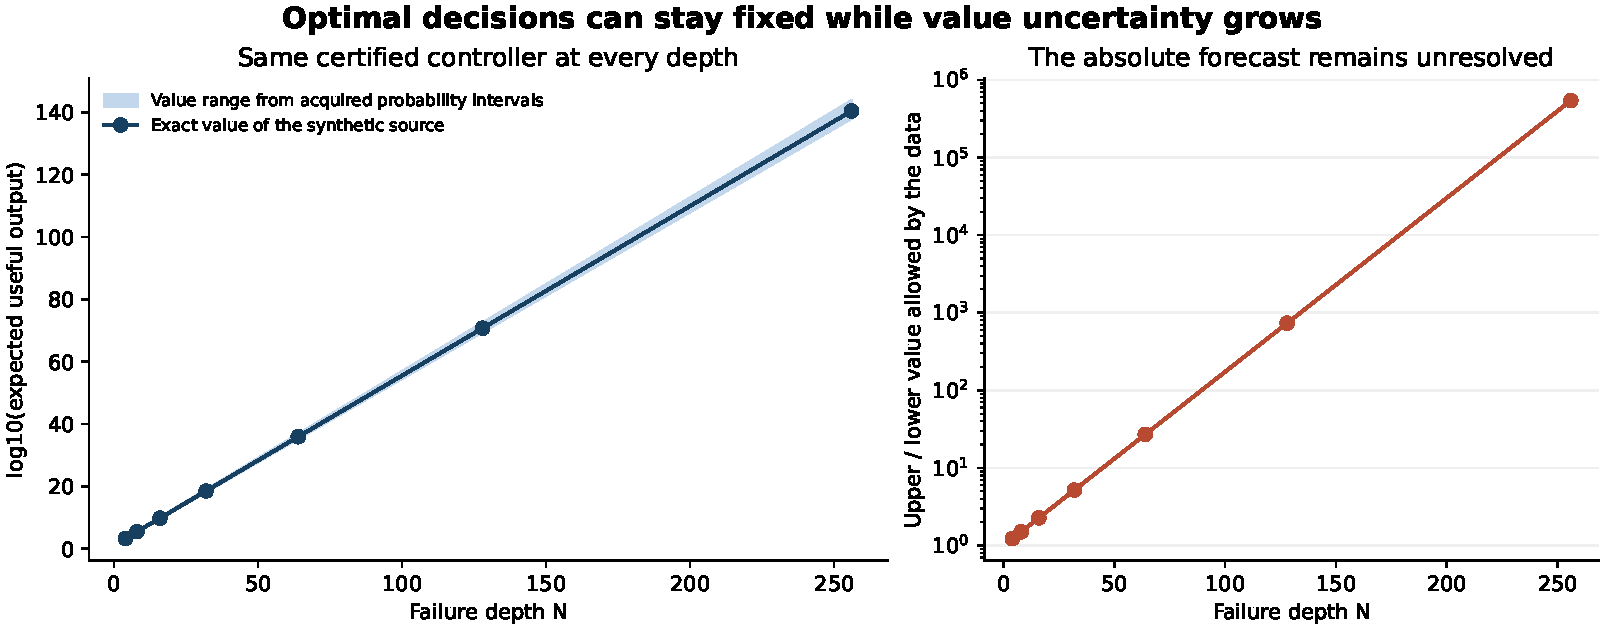
\includegraphics[width=\linewidth]{figures/policy_vs_value.pdf}
\caption{A fixed acquired controller with growing value uncertainty. The shaded interval comes from reported probability bounds. The nominal line uses the diagnostic source, unavailable to the compiler. The wide interval does not itself prove a universal information lower bound.}
\end{figure}

For $N=8$ and 1,000 cycles, the acquired internal-failure upper bound is
$0.01326342$; direct floating propagation gives $0.00910223$. Survival delivers at least 2,000 useful units. The unconditional guarantee also charges $0.01$ calibration risk, initialization error and $1000\eta$ interface risk. For $N=16$, the internal bound for the same mission is approximately $6.9905\,10^{-7}$.

The 742,736 trials and resets are a real sufficient service bill within the model, despite being independent of $N$. No claim of inexpensive hardware or finite-instance sample optimality is made. The asymptotic separation does not guarantee superiority in every small numerical comparison.

\section{Strongest comparison and scientific assessment}

The proper same-decision baseline is direct skip-free dynamic programming with interval or sequential acquisition, together with structural policy-identification methods. It can use the same finite inequalities, inherits the same physical-access conditions and can match or improve the acquisition constants. A comparison only with brute-force catastrophic waiting or unnecessary full trajectory reconstruction would be misleading.

Wijngaard and Stidham~\cite{wijngaard} explicitly describe maximum-total-reward forward recursion for skip-free-to-the-right processes. Serfozo~\cite{serfozo} analyzes controlled random walks and queues with monotone policies. Zanette, Kochenderfer and Brunskill~\cite{zanette} give structure-aware policy identification with generative access in discounted MDPs and strong horizon-related improvements for suboptimal actions. That work precludes claiming the broad idea that policy learning can exploit structure as new. Its discounted conditions are not silently equated to the present undiscounted all-depth certificate.

Chen et al.~\cite{chen} establish strong worst-case stochastic-shortest-path sample-complexity bounds and barriers without generative access. Their minimization, additive-error and access quantifiers differ from the current reward-maximization and relative-value comparison. Those general impossibility results are compatible with a cheap certificate on a structured positive-margin family.

The earned conclusion is that stable local action inequalities can certify a complete optimal productive feedback rule while the absolute rare-event value remains statistically demanding. Its mechanism is stability of choices across an uncertainty set, rather than cancellation of a shared invariant probability. The construction also specifies the boundary: unassayed action-specific catastrophes restore rare observation costs; missing preparation, drift control, support protection and total resources cannot be supplied by the action proof.

The mathematical endpoint is complete under its stated interface. An economical physical realization, a general theory covering unassayed failure mechanisms, demonstrated historical novelty and a civilisation-changing consequence remain unestablished. All accepted earlier machinery is preserved at its actual scope.

\begin{thebibliography}{99}
\bibitem{wijngaard} J. Wijngaard and S. Stidham, Jr. (1986), \emph{Forward Recursion for Markov Decision Processes with Skip-Free-to-the-Right Transitions, Part I: Theory and Algorithm}. Mathematics of Operations Research 11(2), 295--308. \href{https://doi.org/10.1287/moor.11.2.295}{doi:10.1287/moor.11.2.295}.
\bibitem{serfozo} R. Serfozo (1981), \emph{Optimal control of random walks, birth and death processes, and queues}. Advances in Applied Probability 13(1), 61--83. \href{https://doi.org/10.2307/1426467}{doi:10.2307/1426467}.
\bibitem{zanette} A. Zanette, M. J. Kochenderfer and E. Brunskill (2019), \emph{Almost Horizon-Free Structure-Aware Best Policy Identification with a Generative Model}. NeurIPS 32. \href{https://papers.neurips.cc/paper_files/paper/2019/file/a724b9124acc7b5058ed75a31a9c2919-Paper.pdf}{Primary paper}.
\bibitem{chen} L. Chen, A. Tirinzoni, M. Pirotta and A. Lazaric (2023), \emph{Reaching Goals is Hard: Settling the Sample Complexity of the Stochastic Shortest Path}. ALT, PMLR 201, 310--357. \url{https://proceedings.mlr.press/v201/chen23a.html}.
\bibitem{kaufmann} E. Kaufmann, O. Capp\'e and A. Garivier (2016), \emph{On the Complexity of Best-Arm Identification in Multi-Armed Bandit Models}. JMLR 17, 1--42. \href{https://www.jmlr.org/papers/volume17/kaufman16a/kaufman16a.pdf}{Primary paper, especially Lemma 1}.
\bibitem{garivier} A. Garivier and E. Kaufmann (2016), \emph{Optimal Best Arm Identification with Fixed Confidence}. COLT, PMLR 49, 998--1027. \url{https://proceedings.mlr.press/v49/garivier16a.html}.
\bibitem{nitinawarat} S. Nitinawarat and V. V. Veeravalli, \emph{Controlled Sensing for Sequential Multihypothesis Testing with Controlled Markovian Observations and Non-Uniform Control Cost}. Primary preprint, revised 2014. \url{https://arxiv.org/abs/1310.1844}.
\bibitem{naor} P. Naor (1956), \emph{On Machine Interference}. JRSS B 18(2), 280--287. \href{https://doi.org/10.1111/j.2517-6161.1956.tb00235.x}{doi:10.1111/j.2517-6161.1956.tb00235.x}.
\bibitem{salia} R. N. Salia and M. A. Shashiashvili (1985), \emph{On Palm's Model with a Large Number of Machines and Repairmen}. JRSS B 47(2), 316--322. \href{https://doi.org/10.1111/j.2517-6161.1985.tb01359.x}{doi:10.1111/j.2517-6161.1985.tb01359.x}.
\bibitem{crampes} C. Crampes and J. Renault (2016), \emph{The Repairman Problem Revisited}. Annals of Economics and Statistics 121/122, 7--24. \href{https://doi.org/10.15609/annaeconstat2009.121-122.7}{doi:10.15609/annaeconstat2009.121-122.7}.
\bibitem{p2} Astra P2, \emph{Predictive preparation without equilibration}, 5 November 2026. \href{https://github.com/harjassand/astra-research-knowledge/blob/c11d35bd2e07116e214b4388302595cfedbd770e/research/returns/2026-11-05-p2-predictive-preparation/package/predictive_preparation.md}{Exact governing source at commit c11d35bd2e07116e214b4388302595cfedbd770e}. Complete source retained.
\bibitem{prior} Astra, \emph{Direct Acquired Prevention Without Absolute Forecasts}, 5 November 2026. Complete original report, proofs, programs, independent routes and nested first-event package retained in the unchanged ZIP. Its earlier first-event governing revision is \texttt{719e201332992002528c221c49f80f69431485f6}.
\end{thebibliography}
\end{document}


